\documentclass{book}
\usepackage{commeunjeustyle}
\begin{document}


\chapter*{Déterminant}


Dans cette section, on étudie le cas où l'espace de départ et l'espace d'arrivée sont identiques : $f : E\to E$ est un
endomorphisme. Si $\dim E = n$, alors chaque matrice associée à $f$ est une matrice carrée de taille $n$.
\subsection{Déterminant}
\impo{Point de vue géométrique} : dans le plan, le déterminant, $\det$, est une application permettant de calculer l'aire orientée du parallélogramme défini par deux vecteurs, $\Vect{u},\Vect{v}$  
\begin{center}
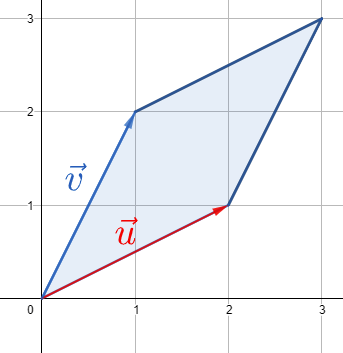
\includegraphics[width=3cm]{determinant.png}
\end{center}
On peut démontrer que l'aire orientée du parallélogramme est donnée par:  
$$
\Fonction{\det}{\R^2\times\R^2}{\R}{((x_1,y_1),(x_2,y_2))}{\begin{vmatrix}
x_1 & x_2 \\
y_1 & y_2
\end{vmatrix}=x_1y_2-y_1x_2}.
$$
Le signe du déterminant s'interprète comme le signe de l'angle orienté entre les deux vecteurs. La valeur absolue du déterminant donne l'aire du parallélogramme engendré. Ceci se révèle crucial dans
différents domaines des mathématiques, par exemple en analyse pour obtenir une formule de changement de variable pour les intégrales doubles.\\
On souhaite étendre l'application déterminant pour calculer le volume d'un parallélépipèdes défini par trois vecteurs dans l'espace : $\det(\Vect{u},\Vect{v},\Vect{w}).$
\begin{center}
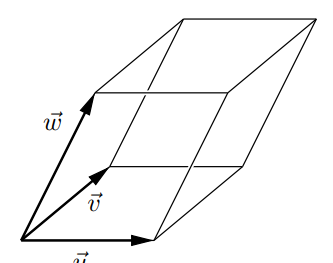
\includegraphics[width=3cm]{determinant3.png}
\end{center}
L'idée fondamentale est de prolonger l'application  déterminant dans le plan à partir de ses propriétés.\\ 
Sur le plan, on remarque que cette application est :
\begin{enumerate}
\item \defi{Normalisé} : l'aire du carré unité est 1, $\det(\Vect{e_1},\Vect{e_2})=1$
\item \defi{2-linéaire} : linéaire par rapport à chaque une de ces deux variables.
\begin{center}
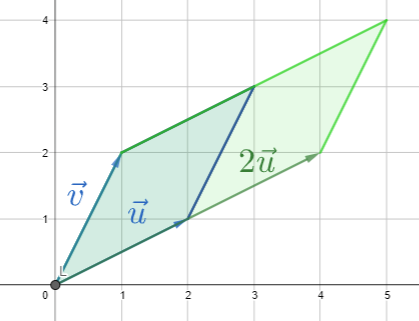
\includegraphics[width=3cm]{determinant2.png}
\end{center}
\item \defi{Alternée} : l'aire d'un parallélogramme aplati est 0, $\det(\Vect{u},\Vect{v})=0$ si $\Vect{u}=\Vect{v}.$
\end{enumerate}
Donc dans l'espace, cette application devrait être :
\begin{enumerate}
\item \defi{Normalisé} : le volume du cube unité est 1, $\det(\Vect{e_1},\Vect{e_2},\Vect{e_3})=1$
\item \defi{3-linéaire} : linéaire par rapport à chaque une de ces trois variables.
\item \defi{Alternée} : le volume d'un parallélépipèdes aplati est 0,  $\det(\Vect{u},\Vect{v},\Vect{w})=0$ si $\Vect{u}=\Vect{v}$ ou $\Vect{u}=\Vect{w}$ ou $\Vect{v}=\Vect{w}$.
\end{enumerate}
Un théorème important est qu'il existe une unique application respectant ces propriétés quelque soit la dimension.\\
Dans la suite, les vecteurs sont rangés sous forme d'une matrice, par exemple $\det((x_1,y_1),(x_2,y_2))=\det(\begin{pmatrix}
x_1 & x_2 \\
y_1 & y_2
\end{pmatrix}).$ 


%Cette \href{https://www.youtube.com/watch?v=Ip3X9LOh2dk}{vidéo de la chaine 3Blue1Brown}
% est une très bonne introduction de la notion de déterminant dans le plan et l'espace. 
 

\begin{Theoreme}[Unicité et existence du déterminant]
Soit $n\in  \N^*$.
Il existe une unique application $\det: \MnK\to\K$ vérifiant les propriétés suivantes:
\begin{enumerate}
\item $\det(\mathrm{I}_n) = 1$;
\item
  $\det(A) = 0$ si deux colonnes de $A$ sont égales;
\item
  Si on fixe $n-1$ colonnes de $A$, l'application qui à la dernière colonne associe $\det(A)$ est linéaire.
  $$\lambda \det(C_1 \dots C_i \dots C_n) + \mu  \det(C_1 \dots C'_i \dots C_n) = \det(C_1 \dots  \lambda C_i+ \mu C'_i  \dots C_n).$$
\end{enumerate}
\end{Theoreme}
\begin{Proposition}[Propriétés]
Cette application $\det$ vérifie alors automatiquement les propriétés suivantes:
\begin{enumerate}
\item \defi{antisymétrique } : 
  $$\det(C_1 \dots C_i \dots C_j  \dots C_n) = -\det(C_1 \dots C_j \dots C_i  \dots C_n)\text{ si }i\neq j$$
\item \defi{stable par combinaison linéaire} :
  $$\det(C_1 \dots C_i  \dots C_n) =\det(C_1 \dots C_i+\lambda C_j  \dots C_n)\text{ si }i\neq j$$
\item \defi{homothétie d'une colonne} :
  $$\det(C_1 \dots \lambda C_i  \dots C_n) =\lambda\det(C_1 \dots C_i  \dots C_n)$$
  En particulier,
  $$\det(\lambda A) =\lambda^n\det(A)$$
\item  \defi{stable par transposition} $$\det (A) = \det (\transposee{A})$$
\item  \defi{multiplication} $$\det (AB) = \det (A)\det(B)$$
\item  \defi{inversible}  $\det(A) \neq 0$ si et seulement si $A$ est inversible. Si $A$ est inversible, son inverse est donnée par :
$$ A^{-1}=\frac {1}{\det A} {\transposee{\text{com}A}}$$
où $\transposee{\text{com}A}$ est la transposée de la comatrice de $A$.
\end{enumerate}
Dans toutes les propriétés précédentes, on peut remplacer les opération sur les colonnes par des opération sur les lignes.
\end{Proposition}
\begin{Proposition}[Matrice triangulaire] Le déterminant d'une matrice triangulaire,$\begin{pmatrix}a_{11}&a_{12}&\cdots &\cdots &a_{1n}\\0&a_{22}&&&a_{2n}\\\vdots &\ddots &\ddots &&\vdots \\\vdots &&\ddots &\ddots &\vdots \\0&\cdots &\cdots &0&a_{nn}\\\end{pmatrix}$,  est égale au produit des coefficients de la diagonale, soit $a_{11}\times a_{22} \times\dots\times a_{nn}$.
\end{Proposition}
\begin{Definition}[Déterminant d'un endomorphisme]
Soit $E$ un $\K $-espace vectoriel de dimension finie et $u$ un endomorphisme de $E$.\\
Soit $\mathcal{B}$ une base de $E$ et $M$ la matrice de $u$ dans la base $\mathcal{B}$.\\
La quantité $\det(M)$ ne dépendant pas du choix de la base $\mathcal{B}$, mais seulement de $u$, on l'appelle \defi{déterminant} de l'endomorphisme $u$ et on note $\det(u) = \det(M)$.
\end{Definition}
\begin{Exemple}[Déterminant de Vandermonde]

Soit $a_1,\dots,a_n \in  \K ^n$.
La \defi{matrice de Vandermonde} associée à $(a_1,\dots,a_n)$ est
\[ M = \begin{pmatrix}
    1 &  1 &  1 &  \dots &  1  \\
    a_1 &  a_2 &  a_3 &  \dots &  a_n  \\
    a_1^2 &  a_2^2 &  a_3^2 &  \dots &  a_n^2  \\
    \vdots &  \vdots &  \vdots &   &  \vdots  \\
a_1^{n-1} &  a_2^{n-1} &  a_3^{n-1} &  \dots &  a_n^{n-1}  \end{pmatrix}. \]
Le \defi{déterminant de Vandermonde} $V(a_1,\dots,a_n)$ est le déterminant de la matrice de Vandermonde ci-dessus. On a :
$$V(a_1,\dots,a_n) = \prod_{1\leq i < j\leq n} (a_j - a_i). $$
En particulier,
\begin{itemize}
\item $V(a) = 1$,
\item $V(a,b) = b-a$,
\item $V(a,b,c) = (b-a)(c-a)(c-b)$.
\end{itemize}
La matrice de Vandermonde associée à $(a_1,\dots,a_n)$ est inversible si et seulement si les nombres $(a_1,\dots,a_n)$ sont deux à deux distincts.
\end{Exemple}








\end{document}
